\section{Poisson equation with PETSc}
  \label{section:applications:petsc}

\chapterDescription
  {
    60 minutes.
  }
  {
    Chapter \ref{chapter:quickstart} and a working PETSc installation.
  }

I wrote Peano with matrix-free methods for computational fluid dynamics in mind. 
It turns out that it is not too complicated to use it for other application
areas or to established linear algebra packages.
We assume that you have PETSc plus BLAS, Lapack and MPI (if required) ready
installed on your system.
I have tested all the present concepts with PETSc 3.7.2 but everything discussed
here is pretty basic, so it should work with older versions as well.
Please note that this is a feasibility study and we do not optimise at all.


\subsection{Preparation of Peano}

If we use explicit assembly, we need an enumeration of our grid. 
So we do start with a grid
\begin{code}
> java -jar <mypath>/pdt.jar --create-project petsc chapter-4.3
\end{code}

\noindent
and add each vertex an index. 
We do restrict to a discretisation with one degree of freedom per vertex for the
time being:

\begin{code}
Packed-Type: short int;

class petsc::records::Vertex {  
  parallelise persistent int index;
};
\end{code}

\noindent
For the present exercise, we will have four different things to do:
create the grid, create and assemble the matrix, solve the problem and plot the
result.
The solve is a pure PETSc operation.
For each of the remaining three phases, we need a mapping/adapter in Peano and
we also want access to \texttt{index}.
For the latter, we could write setters and getters and stick to an
object-oriented paradigm.
But this way, it is easier (though not as beautiful):

\begin{code}
component: MyFancyPETScProject

namespace: ::petsc

vertex:
  dastgen-file: Vertex.def
  read scalar(int): Index   // mind the uppercase
  write scalar(int): Index
  
cell:
  dastgen-file: Cell.def

state:
  dastgen-file: State.def

event-mapping:
  name: CreateGrid

event-mapping:
  name: Assemble

adapter:
  name: CreateGrid
  merge-with-user-defined-mapping: CreateGrid

adapter:
  name: Assemble
  merge-with-user-defined-mapping: Assemble
 
adapter:
  name: Plot
  merge-with-predefined-mapping: VTKPlotVertexValue(result,getU,u)
\end{code}

We generate all glue code
\begin{code}
> java -jar <mypath>/pdt.jar --generate-gluecode \
  petsc/project.peano-specification petsc <mypath>/pdt/usrtemplates
> make -f petsc/makefile
\end{code}

\noindent
We recognise that this code does not compile yet as we have not yet realised \texttt{double Vertex::getU() const}.
For the time being, we make the routine return 0.
Finally, we change into the mapping the creational events yield a regular grid:

\begin{code}
void petsc::mappings::CreateGrid::createInnerVertex(...) {
  logTraceInWith6Arguments( "createInnerVertex(...)", ... );

  if (coarseGridVerticesEnumerator.getLevel()<3) {
	fineGridVertex.refine();
  }

  logTraceOutWith1Argument( "createInnerVertex(...)", fineGridVertex );
}


void petsc::mappings::CreateGrid::createBoundaryVertex(...) {
  logTraceInWith6Arguments( "createBoundaryVertex(...)", ... );

  if (coarseGridVerticesEnumerator.getLevel()<3) {
	fineGridVertex.refine();
  }

  logTraceOutWith1Argument( "createBoundaryVertex(...)", fineGridVertex );
}
\end{code}

\noindent
Compile it, run it, visualise the output.


\subsection{Connecting to PETSc}

As PETSc's philosophy is straightforward and modest (they do, e.g.,
not hijack the main), the initialisation and integration are straightforward.
Please note that we stick to serial jobs in the first part of this
section.
Nevertheless, I typically find it easier to use 
the MPI compiler wrapper to translate the code as I faced
issues when I tried to use PETSc without MPI\footnote{Please consult
\url{http://www.mcs.anl.gov/petsc/petsc-current/docs/installation.html#i-dont-want-to-use-mpi}
for the usage with OpenMPI as the \texttt{LD\_LIBRARY\_PATH} has to be set
properly.}.
Luckily, most MPI implementations even are fine if you translate your code with
\texttt{mpiCC} but then skip a run through \texttt{mpirun} and instead invoke
the executable directly.


\begin{enumerate}
  \item Before we start to code with PETSc, we have to make the makefile know
  where PETSc is installed. If you use your own build environment, adopt all
  pathes accordingly. If you use the pre-generated makefile, open it and add
  your PETSc include directory to the search path. Also switch to
  \texttt{mpiCC} as discussed before.
  \begin{code}
    PROJECT_CFLAGS = -DParallel -I/opt/petsc/include 
    PROJECT_LFLAGS = -L/opt/petsc/lib -lpetsc 
    [...]
    CC=mpiCC
  \end{code}
  Depending on your MPI version, you 
  might run into issues with the compiler's error management if you stick to
  the variants set by Peano's PDT.
  I recommend to
  remove \texttt{-Werror -pedantic-errors} from your makefile in this case.
%   \item As the present PETSc solutions use MPI (through they run serially), we
%   have to make a few modifications in the runner. These modifications are
%   detailed in Chapter \ref{section:parallelisation:mpi}, so we simply show
%   what has to be changed in \texttt{runners/Runner.cpp}. This solution should
%   work out-of-the-box.
%   For a description of its semantics, please see the aforementioned chapter.
%   \begin{code}
% #include "tarch/parallel/FCFSNodePoolStrategy.h"
% #include "peano/parallel/loadbalancing/OracleForOnePhaseWithGreedyPartitioning.h"
% 
% [...]
% 
% int petsc::runners::Runner::run() {
%  [...]
%  petsc::repositories::Repository* repository = 
%   petsc::repositories::RepositoryFactory::getInstance().createWithSTDStackImplementation(
%    geometry,
%    tarch::la::Vector<DIMENSIONS,double>(1.0),   // domainSize,
%    tarch::la::Vector<DIMENSIONS,double>(0.0)    // computationalDomainOffset
%   );
%   
% 
%  // This is new because of PETSc:
%  if (tarch::parallel::Node::getInstance().isGlobalMaster()) {
%   tarch::parallel::NodePool::getInstance().setStrategy(
%    new tarch::parallel::FCFSNodePoolStrategy()
%   );
%  }
%  tarch::parallel::NodePool::getInstance().restart();
%  tarch::parallel::NodePool::getInstance().waitForAllNodesToBecomeIdle();
%  peano::parallel::loadbalancing::Oracle::getInstance().setOracle(
%   new peano::parallel::loadbalancing::OracleForOnePhaseWithGreedyPartitioning(false)
%  );
% 
%  [...]
% }
%   \end{code}
  \item We have to initialise and shut down PETSc properly in
  \texttt{main.cpp}:
  \begin{code}
#include "petscsys.h"

[...]

int main(int argc, char** argv) {
  [...]
  PetscInitialize(&argc,&argv,(char*)0,(char*)0);

  int programExitCode = 0;

  if (programExitCode==0) {
    [...]
    petsc::runners::Runner runner;
    programExitCode = runner.run();
  }

  PetscFinalize();
  [...]
}  
  \end{code}
  \item Finally, we should be able to run an empty project once we have
  augmented the \texttt{LD\_LIBRARY\_PATH} by PETSc.
\end{enumerate}
  

\begin{remark}
   According to PETSc's documentation, we could use PETSc's initialisation to
   set up MPI instead of the Peano initialisation. However, Peano's
   initialisation does not check whether MPI has been set up before. 
   Thus, it makes sense to initialise Peano's MPI through
   \texttt{peano::initParallelEnvironment(&argc,&argv)} before you initialise
   PETSc. In return, you should invoke \texttt{PetscFinalize()} before you call
   \texttt{peano::shutdownParallelEnvironment()}.
\end{remark}




\subsection{The algorithmic and realisation blueprint}

Once we have created the grid (and perhaps visualised it), we can start to set
up the PETSc data structures corresponding to the grid, we can call its solver,
and we can finally free everything afterwards.
We stick to the regular case for the time being.
Again, our example solves the problem
\[
-\Delta u = f
\]
on the unit square with a Finite Element 9-point stencil.


Every fine grid vertex in the grid has a right-hand side and a solution entry. 
Different to previous sections, we do not store the $u$ and $f$ values within
the vertex.
Instead, we will make PETSc hold two vectors $u$ and $f$ and
make each vertex hold an index within these vectors, i.e.~each vertex knows
which entry in the two vectors is associated with the vertex.


Here is a high level sketch of what we have to do:
\begin{enumerate}
  \item Create the grid.
  \item Assign each vertex/dof a unique number.
  \item Ensure that the global vectors $u$ and $f$ do exist and also ensure that
  we have a proper matrix data structure for $A$ available. Initialise both of
  them and free them when the program terminates.
  \item Once $A$ and $f$ contain valid values, solve the equation system $Au=f$
  (note that we reuse the symbols $u$ and $f$ from the PDE though they
  represent continuous values there while they are nodal values in the
  implementation).
  \item Finally, we have to ensure that $A$ and $f$ hold the right values,
  i.e.~we have to assemble them.
\end{enumerate}

\noindent
We first ensure that the assembly process (and also the plotter, runner, \ldots)
know the respective data structures.
For convenience, I recommend to move the three important data variables
into \texttt{Vertex.h}:

\begin{code}
#include "petscvec.h"
#include "petscmat.h"


namespace petsc { 
  class Vertex;
      
  // Forward declaration
  class VertexOperations;

  // These are the global vectors that we use to make the adapter communicate
  // with PETSc:
  extern Vec  u;
  extern Vec  f;
  extern Mat  A;
}
\end{code}

\noindent
We also have to add their definition
to \texttt{Vertex.cpp}:

\begin{code}
Vec  petsc::u;
Vec  petsc::f;
Mat  petsc::A;
\end{code}


\subsection{Enumerating the vertices and initialising vectors and the matrix}

If we tie the entries of a vector/matrix to a vertex, we have to assign the
vertices indices.
We have to couple the vertices from our grid to the PETSc unknowns.
For this, we add a field     

\begin{code}
int  _unknownCounter;
\end{code}

\noindent
to the class \texttt{Assemble} and make each fine grid vertex hold a unique
index which is basically the corresponding entry in the $u$ and $f$ vector.

\begin{code}
#include "petsc/VertexOperations.h"

void petsc::mappings::Assemble::beginIteration(
  petsc::State&  solverState
) {
  logTraceInWith1Argument( "beginIteration(State)", solverState );

  _unknownCounter = 0;

  logTraceOutWith1Argument( "beginIteration(State)", solverState);
}

void petsc::mappings::Assemble::touchVertexFirstTime(
  ...
) {
  logTraceInWith6Arguments( "touchVertexFirstTime(...)", ... );

  if (
    fineGridVertex.getRefinementControl()==Vertex::Records::Unrefined
    &&
    fineGridVertex.isInside() // it is not a boundary point
  ) {
    VertexOperations::writeIndex(fineGridVertex,_unknownCounter);
    _unknownCounter++;
  }
  else {
    VertexOperations::writeIndex(fineGridVertex,-1);
  }

  logTraceOutWith1Argument( "touchVertexFirstTime(...)", fineGridVertex );
}
\end{code}

\noindent
Once we know how many unknowns we are handling, we can create our two required
vectors and we can initialise our matrix properly:


\begin{code}
void petsc::mappings::EnumerateUnknowns::endIteration(...) {
  logTraceInWith1Argument( "endIteration(State)", solverState );

  const PetscInt numberOfUnknowns = _unknownCounter;

  PetscErrorCode errorU = VecCreate(tarch::parallel::Node::getInstance().getCommunicator(), &u);
  PetscErrorCode errorF = VecCreate(tarch::parallel::Node::getInstance().getCommunicator(), &f);

  if (errorU!=0) {
    PetscError( tarch::parallel::Node::getInstance().getCommunicator(),
      __LINE__,  __FUNCT__,  __FILE__, errorU,  PETSC_ERROR_INITIAL,
      "creating global solution vector failed" );
  }
  if (errorF!=0) {
    PetscError( tarch::parallel::Node::getInstance().getCommunicator(),
      __LINE__,  __FUNCT__,  __FILE__, errorF,  PETSC_ERROR_INITIAL,
      "creating global rhs vector failed" );
  }

  VecSetSizes(u, PETSC_DECIDE,numberOfUnknowns);
  VecSetSizes(f, PETSC_DECIDE,numberOfUnknowns);
  VecSetType(u, VECMPI);
  VecSetType(f, VECMPI);
  PetscObjectSetName((PetscObject)u, "Solution");
  PetscObjectSetName((PetscObject)f, "Right-hand side");

  PetscErrorCode errorA = MatCreateSeqAIJ(
    tarch::parallel::Node::getInstance().getCommunicator(),
    numberOfUnknowns,numberOfUnknowns,
    THREE_POWER_D, NULL,
    &A
  );
  if (errorA!=0) {
    PetscError( tarch::parallel::Node::getInstance().getCommunicator(),
      __LINE__,  __FUNCT__,  __FILE__, errorA,  PETSC_ERROR_INITIAL,
      "creating system matrix failed" );
  }

  logTraceOutWith1Argument( "endIteration(State)", solverState);
}
\end{code}


\begin{remark}
 The above snippet where we predefine the number of nonzeros to be $3^d$ per
 row does work only on a regular grid. Adaptive grids might require
 modifications.
\end{remark}


\begin{remark}
 One might be tempted to use the repository's \texttt{getNumberOfInnerVertices}
 routines or similar routines to initialise PETSc.
 This might work, but there are pitfalls: In a distributed memory environment
 these counters might count replicated vertices along domain boundaries twice,
 and the AMR framework cannot know which boundary vertices are real unknowns
 (Neumann, e.g.) and which do not carry unknowns.
\end{remark}



\subsection{Free the data}

Before we continue, we make the runner
destroy all data structures properly:

\begin{code}
int petsc::runners::Runner::runAsMaster(petsc::repositories::Repository& repository) {
  ...
  
  // Clean up PETSc data structures
  VecDestroy(&u);
  VecDestroy(&f);
  MatDestroy(&A);

  repository.logIterationStatistics( true );
  repository.terminate();

  return 0;
}
\end{code}



\subsection{Solve the equation system}


We finally have to solve the actual equation system in the runner. For this, we
plug into the runner snippet above and furthermore include
\texttt{\#include "petscksp.h"}. We use PETSc's default which is a GMRES
and add a Jacobi preconditioner.

\begin{code}
KSP krylovSolver;
PC  preconditioner;

KSPCreate(tarch::parallel::Node::getInstance().getCommunicator(),&krylovSolver);
KSPSetOperators(krylovSolver,A,A); // use matrix from Vector.h

// connect/get preconditioner
KSPGetPC(krylovSolver,&preconditioner);

// set Jacobi as preconditioner
PCSetType(preconditioner,PCBJACOBI);

KSPSolve(krylovSolver,f,u);
KSPDestroy(&krylovSolver);
\end{code}

\noindent
This is not a particular sophisticated code, but it does the job for the time
being.

\begin{remark}
If your application requires $k$ command line arguments, it makes sense to check
that there are at least $k$ arguments and then to let PETSc select a solver
through the command line:
 \begin{code}
KSPCreate(tarch::parallel::Node::getInstance().getCommunicator(),&krylovSolver);
KSPSetFromOptions(krylovSolver);
KSPType krylovSolverType;
KSPGetType(krylovSolver,&krylovSolverType);
logInfo( "run(...)", "use solver " << std::string(krylovSolverType) );
KSPSetOperators(krylovSolver,A,A); // use matrix from Vector.h
 \end{code}
PETSc Krylov solvers are discussed in the PETSc manual in Chapter 4
(\url{http://www.mcs.anl.gov/petsc/petsc-current/docs/manual.pdf#chapter.4}).
I furthermore typically add a 
\begin{code}
int iterations;
KSPGetIterationNumber(krylovSolver, &iterations);
logInfo( "run(...)", "solver terminated after " << iterations << " iteration(s)" );
\end{code}
statements to track the convergence behaviour.
\end{remark}


\subsection{Explicit assembly 2/2: Assembling the right-hand side and the
matrix}

We finally assemble our systems. First, we have to tell
PETSc when we start and when we have finished the assembly.
This matches Peano's idea of a \texttt{beginIteration} and
\texttt{endIteration} event:
 
\begin{code}
void petsc::mappings::Assemble::beginIteration(petsc::State&  solverState) {
  VecAssemblyBegin( u );
  VecAssemblyBegin( f );
  MatAssemblyBegin(A, MAT_FINAL_ASSEMBLY);
}

void petsc::mappings::Assemble::endIteration(petsc::State&  solverState) {
  VecAssemblyEnd( u );
  VecAssemblyEnd( f );
  MatAssemblyEnd(A, MAT_FINAL_ASSEMBLY);
}
\end{code}


\noindent
While the binning of the right-hand side into the matrix is straightforward
(note how we grab the index from the vertex object and then use this index to
write the vector data into the right place)
\begin{code}
void petsc::mappings::Assemble::touchVertexFirstTime(...) {
  if (fineGridVertex.isUnknown()) {
    fineGridVertex.setRhs(
      ...
    );
  }
}

bool petsc::Vertex::isUnknown() const {
  return _vertexData.getIndex()>=0;
}

void petsc::Vertex::setRhs(double rhs) {
  PetscInt     indices[] = {_vertexData.getIndex()};
  PetscScalar  values[]  = {rhs};
  VecSetValues(f,1,indices,values, INSERT_VALUES);
}
\end{code}

\noindent
we have to break down the assembly of the matrix element-wisely:

\begin{code}
#include "tarch/la/Matrix.h"

void petsc::mappings::Assemble::enterCell(...) {
 tarch::la::Matrix<4,4,double> localA;
 localA =  1.0,  -0.5, -0.5,  0.0,
          -0.5,   1.0,  0.0, -0.5,
          -0.5,   0.0,  1.0, -0.5,
           0.0,  -0.5, -0.5,  1.0;

 for(int ii=0; ii<4; ii++)
 for(int jj=0; jj<4; jj++) {
  if (
   fineGridVertices[fineGridVerticesEnumerator(ii)].isUnknown()
   and
   fineGridVertices[fineGridVerticesEnumerator(jj)].isUnknown()
  ) {
   PetscInt row = VertexOperations::readIndex( 
     fineGridVertices[fineGridVerticesEnumerator(ii)] );
   PetscInt col = VertexOperations::readIndex( 
     fineGridVertices[fineGridVerticesEnumerator(jj)] );
   MatSetValue(A,row,col,localA(ii,jj),ADD_VALUES);
  }
 }
}
\end{code}

\noindent
Once you have filled the matrix with entries, you might wanna visualise the
content in the runner with
\begin{code}
  MatView(A,PETSC_VIEWER_STDOUT_WORLD);
  MatView(A,PETSC_VIEWER_DRAW_WORLD);
  std::cin.get();
\end{code}

\pagebreak


\begin{center}
  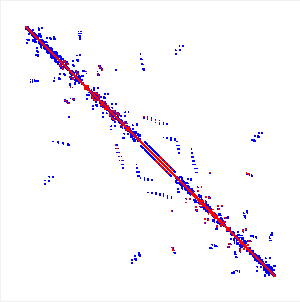
\includegraphics[width=0.4\textwidth]{43_dg/matrix-pattern.png}
  \\
  {
  \footnotesize
  It is important to remember that Peano uses a space-filling curve to traverse
  the grid but can switch to regular subgrids if it deems to be suitable. As a
  consequence, the sparsity pattern even for regular grids might not equal the
  expected $k$-diagonal matrix pattern.
  }
\end{center}

\begin{remark}
  If you know the stencils associated to your vertices, you might prefer to use
  \texttt{matrixfree::stencil::getElementWiseAssemblyMatrix} from Peano's
  \texttt{matrixfree} toolbox which extracts the element-wise stiffness matrix
  from the stencils.
\end{remark}


\subsection{Retrieve properties from the PETSc data structures}

There are many technical ways to couple the vertex to PETSc and to retrieve
data from the explicit assembly.
We do it via the vertices:

\begin{code}
double petsc::Vertex::getU() const {
  double result = 0.0;
  if (_vertexData.getIndex()>=0) {
    PetscInt     indices[] = {_vertexData.getIndex()};
    PetscScalar  values[]  = {0.0};

    VecGetValues(u,1,indices,values);

    result = values[0];
  }
  return result;
}
\end{code}



% 
% \noindent
% Needless to say, this is a 2d example. 3d requires more indices. You might want
% to have a look into the Peano utilities for dimension-generic routines. And it
% is also obvious that this is not a very elegant and fast solution as we write
% into the matrix entry by entry rather than in batches.
% 
% Once the matrix is assembled, it makes sense to add statements alike
% \begin{code}
%   KSPCreate(tarch::parallel::Node::getInstance().getCommunicator(),&krylovSolver);
%   KSPSetOperators(krylovSolver,A,A); // use matrix from Vector.h
% \end{code}
% 
% \noindent
% into the runner to see the matrix pattern, e.g.
% 
% 
% 
% \subsection{Some remarks on discontinuous Galerkin}
% 
% 
% \begin{figure}
%   \begin{center}
%     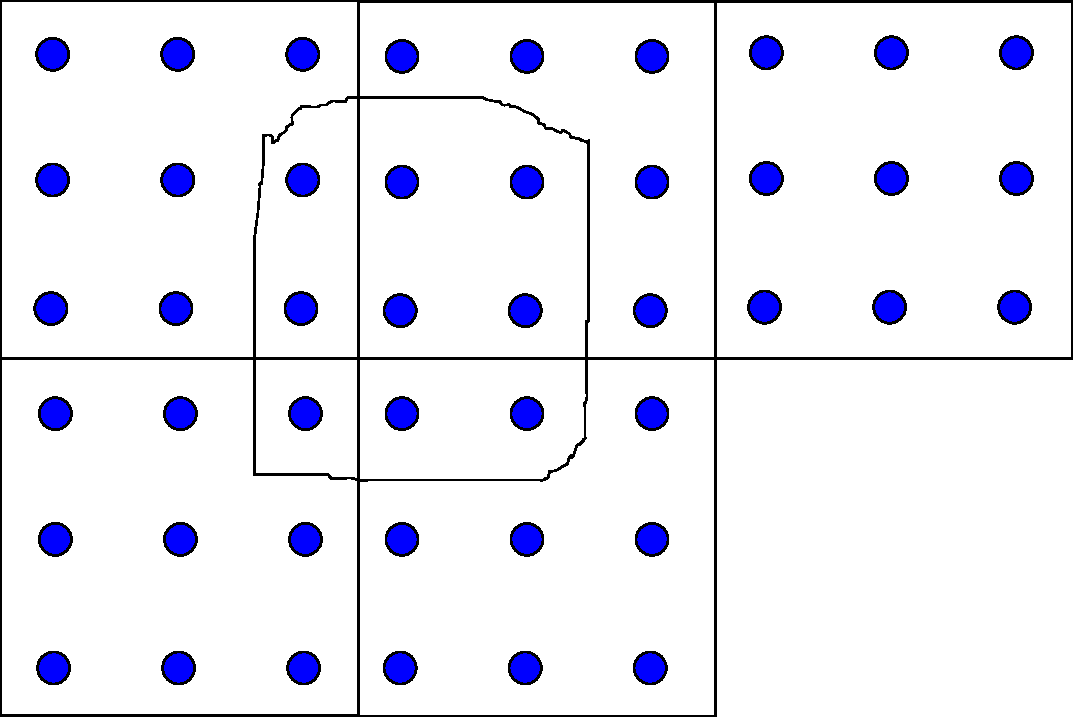
\includegraphics[width=0.6\textwidth]{43_dg/dg-data-layout.pdf}
%   \end{center}
%   \caption{One possible data layout for DG with PETSc. All indices are stored
%   within vertices.}
%   \label{figure:43_petsc:data-layout}
% \end{figure}
% 
% There are various ways to implement discontinuous Galerkin in Peano. 
% We sketch a vertex-based variant  at
% hands of bi-quadratic shape functions.
% For such an approach, we have to store nine unknown per cell.
% However, we propose not to store indices within a cell but within vertices.
% This is advantageous as we have, without additional effort, only vertices within
% a cell at hand. 
% We do not know neighbour cells.
% 
% So we propose to hold nine integer indices within each individual vertex.
% Basically, every unknown is stored within its closest neighbouring vertex
% (Figure \ref{figure:43_petsc:data-layout}). 
% For those where multiple options do exist, we store it to the left bottom.
% The corresponding vertex data structure reads as follows:
% \begin{code}
% Packed-Type: short int;
% 
% class petsc::records::Vertex {  
%   parallelise persistent int index[9];
% };
% \end{code}
% 
% 
% 
% \subsection{Work in progress \ldots}
% 
% I am planning to start some programming with PETSc plus Peano plus MPI soon and
% I also plan to dive into PETSc's matrix-free routines. If anybody reads this
% comment and has suggestions, feel free to contact me.
% 
% \ldots to be continued
% 
% 
% 
% \subsection*{Further reading}
% 
% \begin{itemize}
%   \item Weinzierl, Marion and Weinzierl, Tobias: {\em Quasi-matrix-free hybrid
%   multigrid on dynamically adaptive Cartesian grids}, arXiv:1607.00648
% \end{itemize}
